\begin{frame}
  \frametitle{Evaluation: 23K pages budget}
  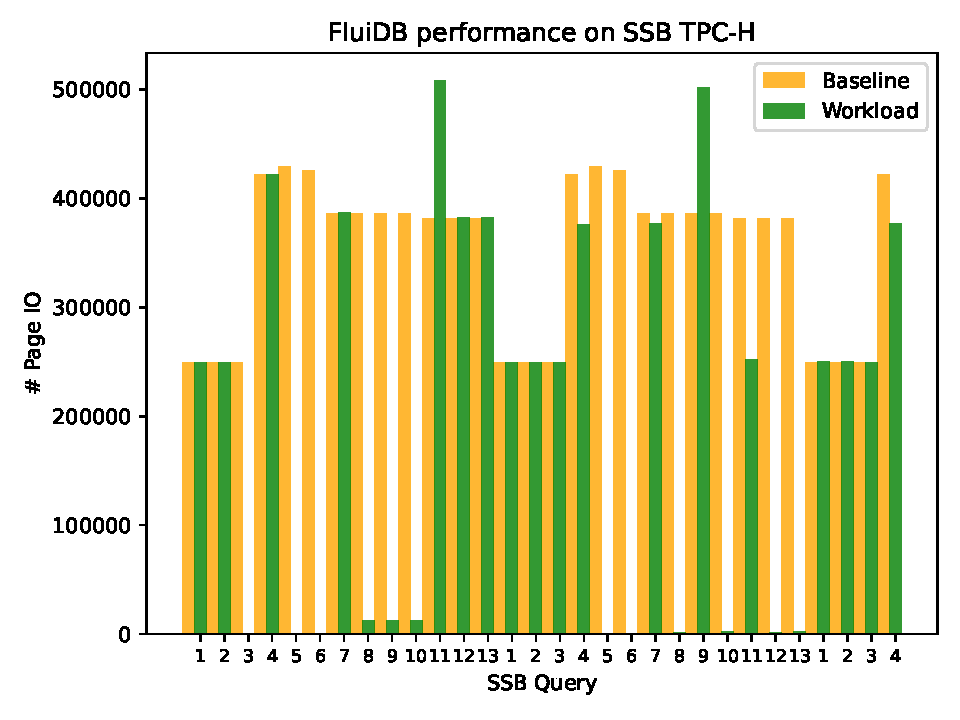
\includegraphics[width=.9\linewidth]{../plans/io_perf_23000.pdf}
\end{frame}

\begin{frame}
  \frametitle{Evaluation: 65K pages budget}
  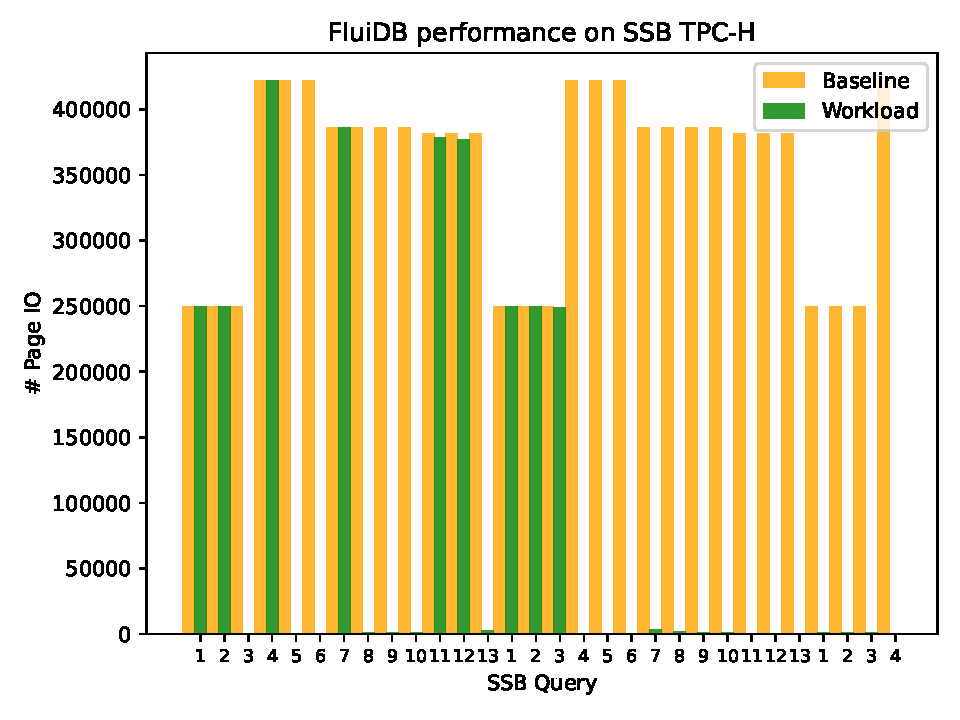
\includegraphics[width=.9\linewidth]{../plans/io_perf_65000.pdf}
\end{frame}

\begin{frame}
  \frametitle{Evaluation: But ... 61K pages budget}
  \framesubtitle{lineorder is deleted at 6 because all join outputs were materialized}
  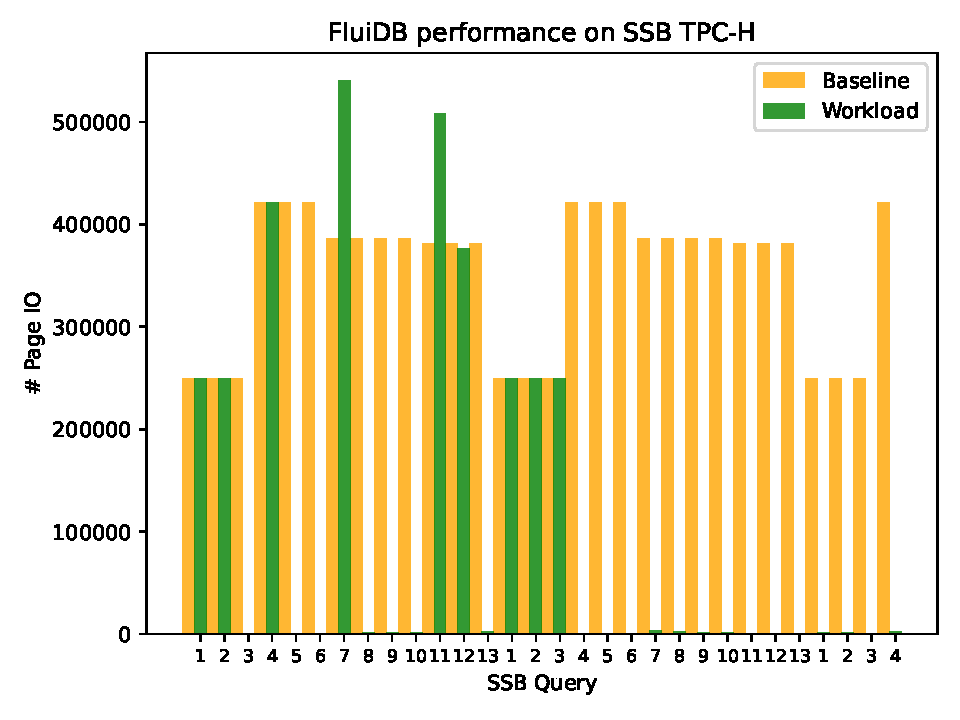
\includegraphics[width=.9\linewidth]{../plans/io_perf_61000.pdf}
\end{frame}

\begin{frame}
  \frametitle{Having enough rope rope}

  \texttt{Demonstrate that all being able to materialize all outputs
    of a join allows us to delete the inputs that may be useful.}
\end{frame}
